\documentclass[a4paper]{article}
\usepackage[left=2.1cm, right=2.1cm, top=2.1cm]{geometry}
\usepackage{lipsum}
\usepackage{tikzpagenodes}
\usepackage{pgfplots}
\usepackage{tikz}
\usepackage{tikz-3dplot}
\usetikzlibrary{arrows,decorations.pathmorphing,backgrounds,positioning,fit,matrix}
\pgfplotsset{compat=1.8}
\usepackage{graphics} % for pdf, bitmapped graphics files
\usepackage{epsfig} % for postscript graphics files
\usepackage[colorlinks=true,citecolor=green]{hyperref}
\usepackage{cite}
\usepackage{amsmath,amssymb,amsfonts}
\usepackage{algorithmic}
\usepackage{graphicx}
\usepackage{url}
\usepackage{cite}
\usepackage{bm}
\usepackage{pbox}
\usepackage{siunitx,booktabs,etoolbox}
\usepackage{ulem}
\usepackage[framed,numbered,autolinebreaks,useliterate]{mcode}
\usepackage{filecontents}
%\usepackage{bigfoot} % to allow verbatim in footnote


\def\BibTeX{{\rm B\kern-.05em{\sc i\kern-.025em b}\kern-.08em
    T\kern-.1667em\lower.7ex\hbox{E}\kern-.125emX}}


\begin{document}

\title{Exercise on Two Image Stiching}
\author{xiahaa@space.dtu.dk}
\maketitle%%

In this exercise, you will work on using all algorithms you have developed yet to do the stiching for two images.

\section{Key Steps}
In order to finish this task, you can follow the following steps:
\begin{enumerate}
\item load two images, do feature (Harris or FAST or SIFT) detection and feature description using Brief 256 or SIFT.
\item Do feature matching. 
\item Use RANSAC and DLT for homography estimation and outlier removal. You can verify your result by plotting all inlier matches. Correct result should show similar match patterns.
\item Do image warping the homography computed using all inliers.
\item Blend the final image to get smooth result.
\end{enumerate}


\begin{figure*}[!b]
	\centering
	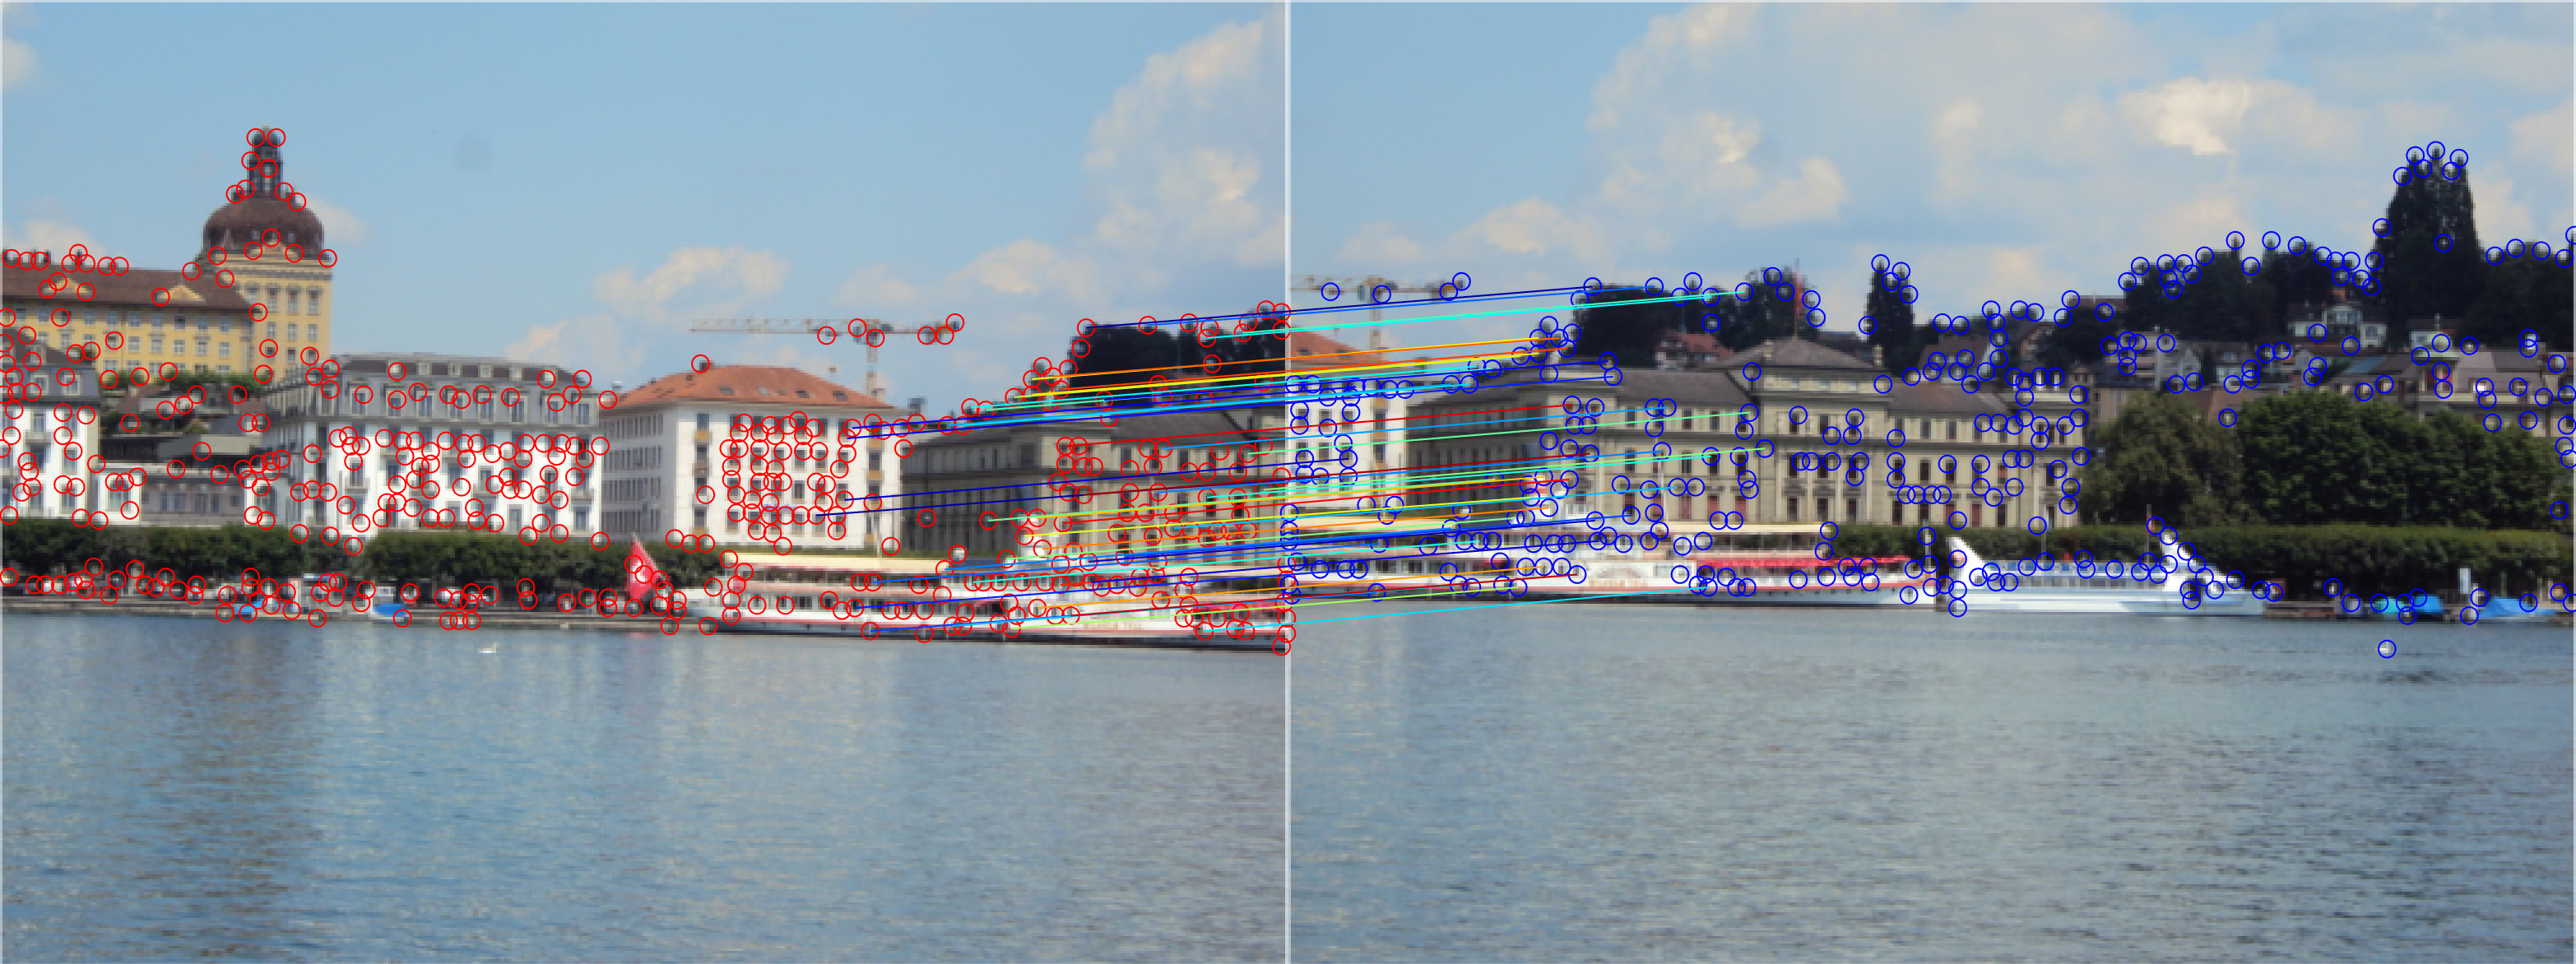
\includegraphics[scale=0.5]{figures/inlier_matches.png}
	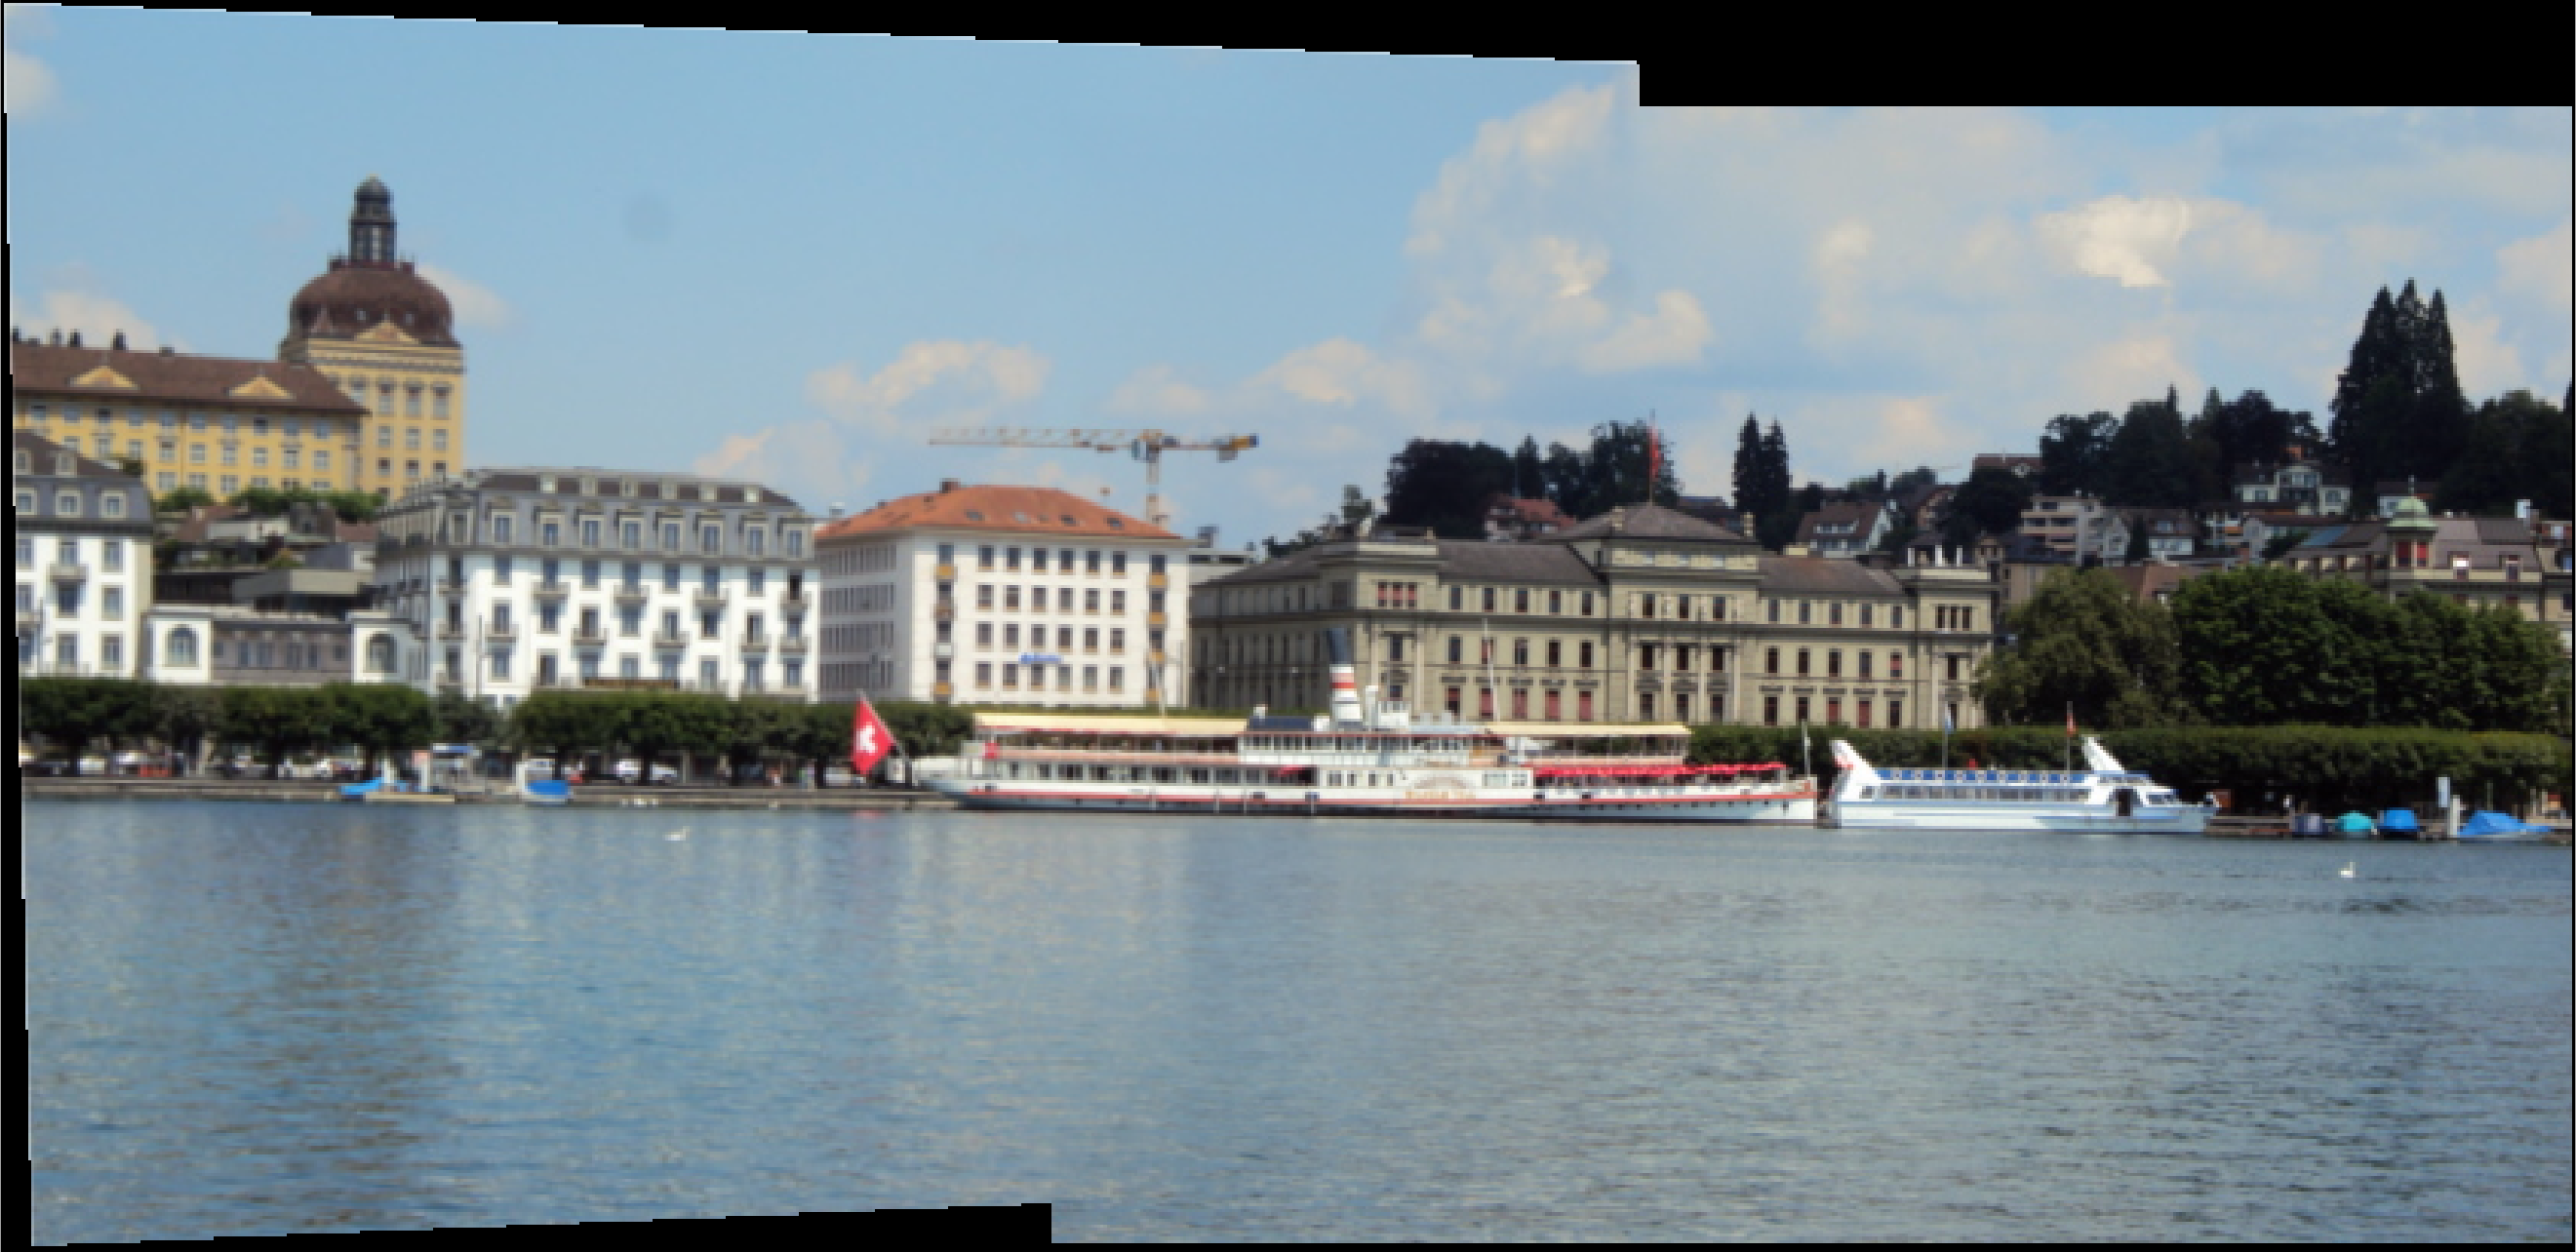
\includegraphics[scale=0.5]{figures/stcih_blend.png}
	\caption{Example of image stich result.}
\end{figure*}

\end{document}